\begin{figure}[ht]
    \centering
    \begin{subfigure}[b]{0.45\textwidth}
        \includegraphics[width=\textwidth]{img/approximation/rof/006hepburn.png}
        \caption{$\lambda = 0.06$}
    \end{subfigure}
    \begin{subfigure}[b]{0.45\textwidth}
        \includegraphics[width=\textwidth]{img/approximation/rof/007hepburn.png}
        \caption{$\lambda = 0.07$}
    \end{subfigure}
    \begin{subfigure}[b]{0.45\textwidth}
        \includegraphics[width=\textwidth]{img/approximation/rof/009hepburn.png}
        \caption{$\lambda = 0.09$}
    \end{subfigure}
    \begin{subfigure}[b]{0.45\textwidth}
        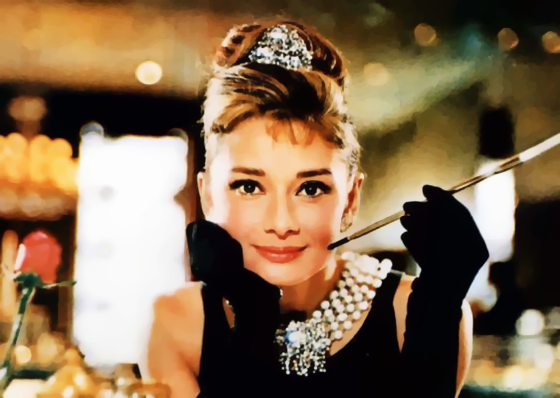
\includegraphics[width=\textwidth]{img/approximation/rof/01hepburn.png}
        \caption{$\lambda = 0.1$}
    \end{subfigure}
    \begin{subfigure}[b]{0.45\textwidth}
        \includegraphics[width=\textwidth]{img/approximation/rof/06hepburn.png}
        \caption{$\lambda = 0.6$}
    \end{subfigure}
    \begin{subfigure}[b]{0.45\textwidth}
        \includegraphics[width=\textwidth]{img/approximation/rof/09hepburn.png}
        \caption{$\lambda = 0.9$}
    \end{subfigure}
    \caption{Approximation of Audrey Hepburn with the ROF Model. The higher $\lambda$ the closer the outcome of the algrithm to the original image.}
\label{fig:rof_hepburn_compare}
\end{figure}

\begin{figure}[ht]
    \centering
    \begin{subfigure}[b]{0.4\textwidth}
        \includegraphics[width=\textwidth]{img/approximation/rof/006lena.png}
        \caption{$\lambda = 0.06$}
    \end{subfigure}
    \begin{subfigure}[b]{0.4\textwidth}
        \includegraphics[width=\textwidth]{img/approximation/rof/007lena.png}
        \caption{$\lambda = 0.07$}
    \end{subfigure}
    \begin{subfigure}[b]{0.4\textwidth}
        \includegraphics[width=\textwidth]{img/approximation/rof/009lena.png}
        \caption{$\lambda = 0.09$}
    \end{subfigure}
    \begin{subfigure}[b]{0.4\textwidth}
        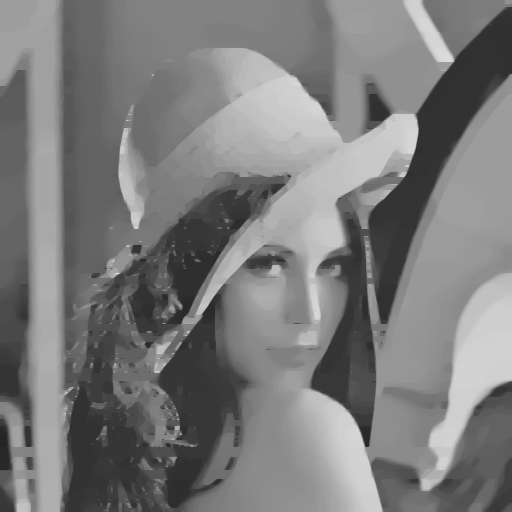
\includegraphics[width=\textwidth]{img/approximation/rof/01lena.png}
        \caption{$\lambda = 0.1$}
    \end{subfigure}
    \begin{subfigure}[b]{0.4\textwidth}
        \includegraphics[width=\textwidth]{img/approximation/rof/06lena.png}
        \caption{$\lambda = 0.6$}
    \end{subfigure}
    \begin{subfigure}[b]{0.4\textwidth}
        \includegraphics[width=\textwidth]{img/approximation/rof/09lena.png}
        \caption{$\lambda = 0.9$}
    \end{subfigure}
    \caption{Approximation of the Lena image with the ROF Model. Again, the higher $\lambda$ the closer the outcome of the algrithm to the original image.}
\label{fig:rof_lena_compare}
\end{figure}

\begin{figure}[ht]
    \centering
    \begin{subfigure}[b]{0.45\textwidth}
        \includegraphics[width=\textwidth]{img/approximation/tvl1/06hepburn.png}
        \caption{$\lambda = 0.6$}
    \end{subfigure}
    \begin{subfigure}[b]{0.45\textwidth}
        \includegraphics[width=\textwidth]{img/approximation/tvl1/07hepburn.png}
        \caption{$\lambda = 0.7$}
    \end{subfigure}
    \begin{subfigure}[b]{0.45\textwidth}
        \includegraphics[width=\textwidth]{img/approximation/tvl1/08hepburn.png}
        \caption{$\lambda = 0.8$}
    \end{subfigure}
    \begin{subfigure}[b]{0.45\textwidth}
        \includegraphics[width=\textwidth]{img/approximation/tvl1/09hepburn.png}
        \caption{$\lambda = 0.9$}
    \end{subfigure}
    \caption{Approximation of Audrey Hepburn with the TVL1 Model. The higher $\lambda$ the closer the outcome of the algrithm to the original image.}
\label{fig:tvl1_hepburn_compare}
\end{figure}

\begin{figure}[ht]
    \centering
    \begin{subfigure}[b]{0.4\textwidth}
        \includegraphics[width=\textwidth]{img/approximation/tvl1/06lena.png}
        \caption{$\lambda = 0.6$}
    \end{subfigure}
    \begin{subfigure}[b]{0.4\textwidth}
        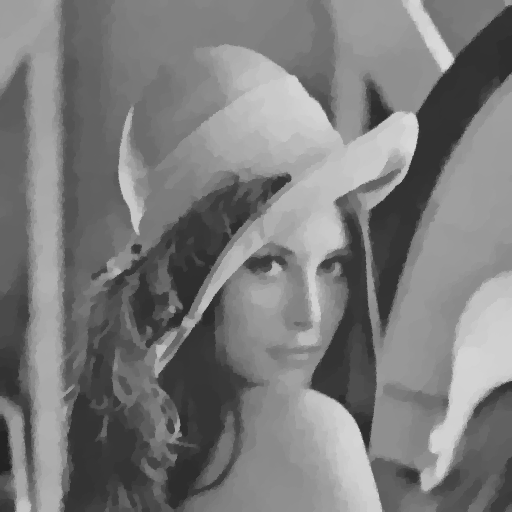
\includegraphics[width=\textwidth]{img/approximation/tvl1/07lena.png}
        \caption{$\lambda = 0.7$}
    \end{subfigure}
    \begin{subfigure}[b]{0.4\textwidth}
        \includegraphics[width=\textwidth]{img/approximation/tvl1/08lena.png}
        \caption{$\lambda = 0.8$}
    \end{subfigure}
    \begin{subfigure}[b]{0.4\textwidth}
        \includegraphics[width=\textwidth]{img/approximation/tvl1/09lena.png}
        \caption{$\lambda = 0.9$}
    \end{subfigure}
    \caption{Approximation of the Lena image with the TVL1 Model. Again, the higher $\lambda$ the closer the outcome of the algrithm to the original image.}
\label{fig:tvl1_lena_compare}
\end{figure}

\begin{figure}[ht]
    \centering
    \begin{subfigure}[b]{0.45\textwidth}
        \includegraphics[width=\textwidth]{img/approximation/realtime/003hepburn20.png}
        \caption{$\alpha = 20, \lambda = 0.03$ (piecewise smooth)}
    \end{subfigure}
    \begin{subfigure}[b]{0.45\textwidth}
        \includegraphics[width=\textwidth]{img/approximation/realtime/05hepburn500.png}
        \caption{$\alpha = 500, \lambda = 0.5$ (piecewise constant)}
    \end{subfigure}
    \begin{subfigure}[b]{0.45\textwidth}
        \includegraphics[width=\textwidth]{img/approximation/realtime/004hepburn20.png}
        \caption{$\alpha = 20, \lambda = 0.04$ (piecewise smooth)}
    \end{subfigure}
    \begin{subfigure}[b]{0.45\textwidth}
        \includegraphics[width=\textwidth]{img/approximation/realtime/07hepburn500.png}
        \caption{$\alpha = 500, \lambda = 0.7$ (piecewise constant)}
    \end{subfigure}
    \caption{Approximation of Audrey Hepburn with the Mumford-Shah Model. The higher $\lambda$ the closer the outcome of the algrithm to the original image.}
\label{fig:realtime_hepburn_compare}
\end{figure}

\begin{figure}[ht]
    \centering
    \begin{subfigure}[b]{0.4\textwidth}
        \includegraphics[width=\textwidth]{img/approximation/realtime/003lena20.png}
        \caption{$\alpha = 20, \lambda = 0.03$ (piecewise smooth)}
    \end{subfigure}
    \begin{subfigure}[b]{0.4\textwidth}
        \includegraphics[width=\textwidth]{img/approximation/realtime/007lena500.png}
        \caption{$\alpha = 500, \lambda = 0.5$ (piecewise constant)}
    \end{subfigure}
    \begin{subfigure}[b]{0.4\textwidth}
        \includegraphics[width=\textwidth]{img/approximation/realtime/004lena20.png}
        \caption{$\alpha = 20, \lambda = 0.04$ (piecewise smooth)}
    \end{subfigure}
    \begin{subfigure}[b]{0.4\textwidth}
        \includegraphics[width=\textwidth]{img/approximation/realtime/008lena500.png}
        \caption{$\alpha = 500, \lambda = 0.7$ (piecewise constant)}
    \end{subfigure}
    \caption{Approximation of the Lena image with the Mumford-Shah Model. Again, the higher $\lambda$ the closer the outcome of the algrithm to the original image.}
\label{fig:realtime_lena_compare}
\end{figure}

\begin{figure}[ht]
    \centering
    \begin{center}
        \rotatebox{90}{$\lambda = 0.005$}
        \begin{subfigure}[b]{0.19\textwidth}
            \includegraphics[width=\textwidth]{img/evolution/rof/0005lena.png}
        \end{subfigure}
        \rotatebox{90}{$\lambda = 0.2$}
        \begin{subfigure}[b]{0.19\textwidth}
            \includegraphics[width=\textwidth]{img/evolution/tvl1/02lena.png}
        \end{subfigure}
        \rotatebox{90}{$\lambda = 0.01$}
        \begin{subfigure}[b]{0.19\textwidth}
            \includegraphics[width=\textwidth]{img/evolution/realtime/001lena20.png}
        \end{subfigure}
        \rotatebox{90}{$\lambda = 0.01$}
        \begin{subfigure}[b]{0.19\textwidth}
            \includegraphics[width=\textwidth]{img/evolution/realtime/001lena500.png}
        \end{subfigure}
    \end{center}
    \begin{center}
        \rotatebox{90}{$\lambda = 0.007$}
        \begin{subfigure}[b]{0.19\textwidth}
            \includegraphics[width=\textwidth]{img/evolution/rof/0007lena.png}
        \end{subfigure}
        \rotatebox{90}{$\lambda = 0.3$}
        \begin{subfigure}[b]{0.19\textwidth}
            \includegraphics[width=\textwidth]{img/evolution/tvl1/03lena.png}
        \end{subfigure}
        \rotatebox{90}{$\lambda = 0.03$}
        \begin{subfigure}[b]{0.19\textwidth}
            \includegraphics[width=\textwidth]{img/evolution/realtime/003lena20.png}
        \end{subfigure}
        \rotatebox{90}{$\lambda = 0.03$}
        \begin{subfigure}[b]{0.19\textwidth}
            \includegraphics[width=\textwidth]{img/evolution/realtime/003lena500.png}
        \end{subfigure}
    \end{center}
    \begin{center}
        \rotatebox{90}{$\lambda = 0.009$}
        \begin{subfigure}[b]{0.19\textwidth}
            \includegraphics[width=\textwidth]{img/evolution/rof/0009lena.png}
        \end{subfigure}
        \rotatebox{90}{$\lambda = 0.4$}
        \begin{subfigure}[b]{0.19\textwidth}
            \includegraphics[width=\textwidth]{img/evolution/tvl1/04lena.png}
        \end{subfigure}
        \rotatebox{90}{$\lambda = 0.05$}
        \begin{subfigure}[b]{0.19\textwidth}
            \includegraphics[width=\textwidth]{img/evolution/realtime/005lena20.png}
        \end{subfigure}
        \rotatebox{90}{$\lambda = 0.05$}
        \begin{subfigure}[b]{0.19\textwidth}
            \includegraphics[width=\textwidth]{img/evolution/realtime/005lena500.png}
        \end{subfigure}
    \end{center}
    \begin{center}
        \rotatebox{90}{$\lambda = 0.02$}
        \begin{subfigure}[b]{0.19\textwidth}
            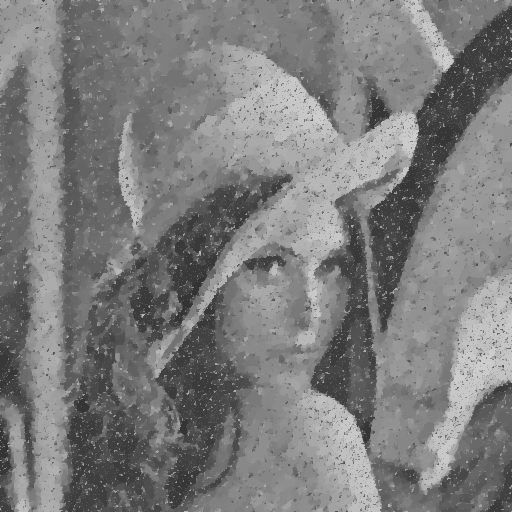
\includegraphics[width=\textwidth]{img/evolution/rof/002lena.png}
        \end{subfigure}
        \rotatebox{90}{$\lambda = 0.5$}
        \begin{subfigure}[b]{0.19\textwidth}
            \includegraphics[width=\textwidth]{img/evolution/tvl1/05lena.png}
        \end{subfigure}
        \rotatebox{90}{$\lambda = 0.07$}
        \begin{subfigure}[b]{0.19\textwidth}
            \includegraphics[width=\textwidth]{img/evolution/realtime/007lena20.png}
        \end{subfigure}
        \rotatebox{90}{$\lambda = 0.07$}
        \begin{subfigure}[b]{0.19\textwidth}
            \includegraphics[width=\textwidth]{img/evolution/realtime/007lena500.png}
        \end{subfigure}
    \end{center}
    \begin{center}
        \rotatebox{90}{$\lambda = 0.04$}
        \begin{subfigure}[b]{0.19\textwidth}
            \includegraphics[width=\textwidth]{img/evolution/rof/004lena.png}
        \end{subfigure}
        \rotatebox{90}{$\lambda = 0.6$}
        \begin{subfigure}[b]{0.19\textwidth}
            \includegraphics[width=\textwidth]{img/evolution/tvl1/06lena.png}
        \end{subfigure}
        \rotatebox{90}{$\lambda = 0.09$}
        \begin{subfigure}[b]{0.19\textwidth}
            \includegraphics[width=\textwidth]{img/evolution/realtime/009lena20.png}
        \end{subfigure}
        \rotatebox{90}{$\lambda = 0.09$}
        \begin{subfigure}[b]{0.19\textwidth}
            \includegraphics[width=\textwidth]{img/evolution/realtime/009lena500.png}
        \end{subfigure}
    \end{center}
    \caption{Evolution of the Lena image, whereas the left column shows the ROF Model, the second column the TVL1 Model, the third column resembles the piecewise smooth approximation of the Mumford-Shah Model with the real-time minimizer with $\alpha = 20$. The right column shows the piecewise constant case of the last mentioned algorithm with $\alpha = 500$.}
\end{figure}

\begin{figure}[ht]
    \centering
    \begin{center}
        \rotatebox{90}{$\lambda = 0.005$}
        \begin{subfigure}[b]{0.21\textwidth}
            \includegraphics[width=\textwidth]{img/evolution/rof/0005hepburn.png}
        \end{subfigure}
        \rotatebox{90}{$\lambda = 0.2$}
        \begin{subfigure}[b]{0.21\textwidth}
            \includegraphics[width=\textwidth]{img/evolution/tvl1/02hepburn.png}
        \end{subfigure}
        \rotatebox{90}{$\lambda = 0.01$}
        \begin{subfigure}[b]{0.21\textwidth}
            \includegraphics[width=\textwidth]{img/evolution/realtime/001hepburn20.png}
        \end{subfigure}
        \rotatebox{90}{$\lambda = 0.1$}
        \begin{subfigure}[b]{0.21\textwidth}
            \includegraphics[width=\textwidth]{img/evolution/realtime/01hepburn500.png}
        \end{subfigure}
    \end{center}
    \begin{center}
        \rotatebox{90}{$\lambda = 0.007$}
        \begin{subfigure}[b]{0.21\textwidth}
            \includegraphics[width=\textwidth]{img/evolution/rof/0007hepburn.png}
        \end{subfigure}
        \rotatebox{90}{$\lambda = 0.3$}
        \begin{subfigure}[b]{0.21\textwidth}
            \includegraphics[width=\textwidth]{img/evolution/tvl1/03hepburn.png}
        \end{subfigure}
        \rotatebox{90}{$\lambda = 0.03$}
        \begin{subfigure}[b]{0.21\textwidth}
            \includegraphics[width=\textwidth]{img/evolution/realtime/003hepburn20.png}
        \end{subfigure}
        \rotatebox{90}{$\lambda = 0.3$}
        \begin{subfigure}[b]{0.21\textwidth}
            \includegraphics[width=\textwidth]{img/evolution/realtime/03hepburn500.png}
        \end{subfigure}
    \end{center}
    \begin{center}
        \rotatebox{90}{$\lambda = 0.009$}
        \begin{subfigure}[b]{0.21\textwidth}
            \includegraphics[width=\textwidth]{img/evolution/rof/0009hepburn.png}
        \end{subfigure}
        \rotatebox{90}{$\lambda = 0.4$}
        \begin{subfigure}[b]{0.21\textwidth}
            \includegraphics[width=\textwidth]{img/evolution/tvl1/04hepburn.png}
        \end{subfigure}
        \rotatebox{90}{$\lambda = 0.05$}
        \begin{subfigure}[b]{0.21\textwidth}
            \includegraphics[width=\textwidth]{img/evolution/realtime/005hepburn20.png}
        \end{subfigure}
        \rotatebox{90}{$\lambda = 0.5$}
        \begin{subfigure}[b]{0.21\textwidth}
            \includegraphics[width=\textwidth]{img/evolution/realtime/05hepburn500.png}
        \end{subfigure}
    \end{center}
    \begin{center}
        \rotatebox{90}{$\lambda = 0.02$}
        \begin{subfigure}[b]{0.21\textwidth}
            \includegraphics[width=\textwidth]{img/evolution/rof/002hepburn.png}
        \end{subfigure}
        \rotatebox{90}{$\lambda = 0.5$}
        \begin{subfigure}[b]{0.21\textwidth}
            \includegraphics[width=\textwidth]{img/evolution/tvl1/05hepburn.png}
        \end{subfigure}
        \rotatebox{90}{$\lambda = 0.07$}
        \begin{subfigure}[b]{0.21\textwidth}
            \includegraphics[width=\textwidth]{img/evolution/realtime/007hepburn20.png}
        \end{subfigure}
        \rotatebox{90}{$\lambda = 0.7$}
        \begin{subfigure}[b]{0.21\textwidth}
            \includegraphics[width=\textwidth]{img/evolution/realtime/07hepburn500.png}
        \end{subfigure}
    \end{center}
    \begin{center}
        \rotatebox{90}{$\lambda = 0.04$}
        \begin{subfigure}[b]{0.21\textwidth}
            \includegraphics[width=\textwidth]{img/evolution/rof/004hepburn.png}
        \end{subfigure}
        \rotatebox{90}{$\lambda = 0.6$}
        \begin{subfigure}[b]{0.21\textwidth}
            \includegraphics[width=\textwidth]{img/evolution/tvl1/06hepburn.png}
        \end{subfigure}
        \rotatebox{90}{$\lambda = 0.09$}
        \begin{subfigure}[b]{0.21\textwidth}
            \includegraphics[width=\textwidth]{img/evolution/realtime/009hepburn20.png}
        \end{subfigure}
        \rotatebox{90}{$\lambda = 0.9$}
        \begin{subfigure}[b]{0.21\textwidth}
            \includegraphics[width=\textwidth]{img/evolution/realtime/09hepburn500.png}
        \end{subfigure}
    \end{center}
    \caption{Evolution of the Audrey Hepburn image, whereas the left column shows the ROF Model, the second column the TVL1 Model, the third column resembles the piecewise smooth approximation of the Mumford-Shah Model with the real-time minimizer with $\alpha = 20$. The right column shows the piecewise constant case of the last mentioned algorithm with $\alpha = 500$.}
\end{figure}